\clearpage
\VerdierPhysicalPageAnchor{0096}%
\begingroup
\setlength{\abovedisplayskip}{3pt plus 2pt minus 2pt}%
\setlength{\belowdisplayskip}{3pt plus 2pt minus 2pt}%
\VerdierSemanticAnchor{ch1-3-3-2-open-morphism-continuation}
de $\operatorname{comp}(C)$ dans la classe modulo homotopie de
$u\colon X\to Y$.
\VerdierSemanticAnchor{ch1-3-3-2-representative}
On a alors un objet de $\operatorname{Tr}_1(C)$ :
$X\xrightarrow{\dot f}Y$.
\VerdierSemanticAnchor{ch1-3-3-2-completion-cone}
Le triangle distingué :
\begin{equation*}
  X\xrightarrow{u}Y\xrightarrow{\dot p(f)}c(f)
  \xrightarrow{\dot q(f)}X[1]
\end{equation*}
\VerdierSemanticAnchor{ch1-3-3-2-completion-conclusion}
contient le morphisme $u$.

\VerdierSemanticAnchor{ch1-3-3-3}
\noindent\textbf{Proposition 3.3.3. (TRII)}\quad
\VerdierSemanticAnchor{ch1-3-3-3-trii}
\textit{Un triangle
$X\xrightarrow{u}Y\xrightarrow{v}Z\xrightarrow{w}X[1]$ de $K(C)$ est
distingué si et seulement si le triangle
$Y\xrightarrow{v}Z\xrightarrow{w}X[1]\xrightarrow{-u[1]}Y[1]$ est
distingué.}

\VerdierSemanticAnchor{ch1-3-3-3-proof-forward}
Supposons que le triangle
$X\xrightarrow{u}Y\xrightarrow{v}Z\xrightarrow{w}X[1]$ soit distingué.
Il est alors isomorphe à un triangle du type :

\VerdierSemanticAnchor{ch1-3-3-3-cone-model}
\begin{equation*}
  X'\xrightarrow{\dot f}Y'\xrightarrow{\dot p(f)}c(f)
  \xrightarrow{\dot q(f)}X'[1],
\end{equation*}
où $X'\xrightarrow{\dot f}Y'$ est un objet de $\operatorname{Tr}_1(C)$.
Il suffit donc de montrer que le triangle :

\VerdierSemanticAnchor{ch1-3-3-3-rotated-model}
\begin{equation*}
  Y'\xrightarrow{\dot p(f)}c(f)\xrightarrow{\dot q(f)}X'[1]
  \xrightarrow{-\dot f[1]}Y'[1],
\end{equation*}
est distingué. Or d'après (3.2.6), le diagramme :

\VerdierSemanticAnchor{ch1-3-3-3-comparison}
\begin{center}
  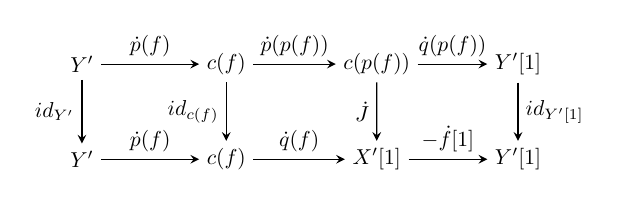
\begin{tikzpicture}[>=stealth,scale=0.78,every node/.style={transform shape}]
    \node (Y1)  at (0,1.55) {$Y'$};
    \node (Cf1) at (2.35,1.55) {$c(f)$};
    \node (Cpf) at (4.80,1.55) {$c(p(f))$};
    \node (Ys1) at (7.10,1.55) {$Y'[1]$};
    \node (Y2)  at (0,0) {$Y'$};
    \node (Cf2) at (2.35,0) {$c(f)$};
    \node (Xs)  at (4.80,0) {$X'[1]$};
    \node (Ys2) at (7.10,0) {$Y'[1]$};
    \draw[->] (Y1) -- node[above] {$\dot p(f)$} (Cf1);
    \draw[->] (Cf1) -- node[above] {$\dot p(p(f))$} (Cpf);
    \draw[->] (Cpf) -- node[above] {$\dot q(p(f))$} (Ys1);
    \draw[->] (Y2) -- node[above] {$\dot p(f)$} (Cf2);
    \draw[->] (Cf2) -- node[above] {$\dot q(f)$} (Xs);
    \draw[->] (Xs) -- node[above] {$-\dot f[1]$} (Ys2);
    \draw[->] (Y1) -- node[left] {$\operatorname{id}_{Y'}$} (Y2);
    \draw[->] (Cf1) -- node[left] {$\operatorname{id}_{c(f)}$} (Cf2);
    \draw[->] (Cpf) -- node[left] {$\dot J$} (Xs);
    \draw[->] (Ys1) -- node[right] {$\operatorname{id}_{Y'[1]}$} (Ys2);
  \end{tikzpicture}
\end{center}

\VerdierSemanticAnchor{ch1-3-3-3-forward-conclusion}
est un isomorphisme de triangles dans $K(C)$.

\VerdierSemanticAnchor{ch1-3-3-3-proof-reverse}
Supposons maintenant que le triangle
$Y\xrightarrow{v}Z\xrightarrow{w}X[1]\xrightarrow{-u[1]}Y[1]$ soit
distingué. On en déduit par (3.2.4) que le triangle :

\VerdierSemanticAnchor{ch1-3-3-3-shifted-triangle}
\begin{equation*}
  Y[-1]\xrightarrow{v[-1]}Z[-1]\xrightarrow{w[-1]}X
  \xrightarrow{u}Y
\end{equation*}
est distingué et,
\VerdierSemanticAnchor{ch1-3-3-3-double-rotation}
en appliquant deux fois l'argument précédent, que le triangle :
\begin{equation*}
  X\xrightarrow{u}Y\xrightarrow{v}Z\xrightarrow{w}X[1]
\end{equation*}
\VerdierSemanticAnchor{ch1-3-3-3-conclusion}
est distingué, ce qui achève la démonstration.
\endgroup

